\documentclass[runningheads]{llncs}

\usepackage[T1]{fontenc}
\usepackage{graphicx}
\usepackage{booktabs}
\usepackage{xcolor}
\usepackage{array}
\usepackage{microtype}
\usepackage{tikz}
\usetikzlibrary{arrows.meta,positioning,shapes.geometric,calc}

\newcolumntype{L}[1]{>{\raggedright\arraybackslash}p{#1}}
\raggedbottom

\usepackage[hidelinks,breaklinks]{hyperref}

\newif\ifdraftnotes
\draftnotestrue         
\newcommand{\PH}[1]{%
  \ifdraftnotes
    \par\noindent\colorbox{black!7}{%
      \parbox{0.97\linewidth}{\footnotesize\textcolor{black!65}{\textsf{[TODO]}~#1}}}\par\medskip
  \fi}
\newcommand{\NUM}[1]{\textcolor{red}{\textbf{#1}}}  
\begin{document}

\title{Evaluation as Supervision: Deterministic Runtime\texorpdfstring{\\}{: }
       Verification of Claims in a Multi-Agent LLM Pipeline}

\titlerunning{Evaluation as Supervision}


\author{
Huu Hoan Hoang \orcidID{0009-0003-6165-0197} \and
Ho Quang Dung Pham\and
Manh Duc Tran \and 
Nam Khanh Nguyen \and
Manh Toan Nguyen\orcidID{0000-0002-9870-8837}
}
\institute{
Swinburne Vietnam, FPT University, Hanoi, Vietnam \\
    \email{\{105732188, 105706604, 104774105, 105706565,\}@student.swin.edu.au}
\email{toannm36@fe.edu.vn}
}
\authorrunning{H.H. Hoang et al.}

\maketitle

% =====================================================================
\begin{abstract}
Structured-output tooling has made large language model (LLM) pipelines reliably
well-formed, but not reliably grounded: a fabricated yet schema-valid output
passes every validation gate such pipelines apply. In a \emph{staged} pipeline,
where every agent consumes only outputs produced earlier in the same run, each
downstream claim has a checkable provenance in upstream state, so groundedness
can be verified deterministically at run time without ground-truth labels. We
exploit this by promoting an offline evaluation harness into a runtime supervisor
that measures each stage with deterministic checks (evidence resolution,
statistic recomputation, cross-stage containment) and routes on hard rules over
those measurements, injecting the measured failure back into the agent's prompt
on retry. We evaluate on a four-agent restaurant review analysis pipeline over
the Yelp Open Dataset, across 20 businesses sampled to span the real
review-count distribution. An unsupervised pipeline emitted at least one
ungrounded claim in 35\% of runs, and those defects proved unstable: on identical
input at temperature~0, a retry-triggering defect reappeared at the same stage in
20\% of runs, so single-run evaluation of such a pipeline reports a draw rather
than a property. We report the measures that are \emph{not} circular with respect
to what the supervisor enforces, and state the derivability precondition under
which the pattern transfers.

\keywords{LLM agents \and hallucination detection \and runtime verification
\and multi-agent systems \and grounding.}
\end{abstract}

% =====================================================================
\section{Introduction}
\label{sec:intro}

Structured output has changed what can go wrong in a large language model
pipeline. The defensive stack built around it --- schema validation, retry on
parse error, model fallback, criticality downgrade --- protects against one
thing: the output being \emph{malformed}. None of it protects against the output
being \emph{wrong}. A
fabricated claim that satisfies its schema parses, validates, and is reported as
success, and in a multi-stage system it becomes the input from which every later
stage reasons.

In a common class of pipeline this failure is detectable with no external
resource. Call a pipeline \emph{staged} when every agent's input consists only of
outputs that earlier agents in the same run produced. Then every claim either
derives from upstream state or was invented by the stage that emitted it, so
verifying groundedness reduces to consistency checking against data the system
already holds --- at run time, with no labels and no second model. We call this
the \emph{derivability property} (Section~\ref{sec:derivability}).

We exploit it by promoting an offline evaluation harness into a runtime
supervisor: it measures each stage deterministically against upstream state,
routes on hard rules over those measurements, and on retry writes the measured
failure into the prompt of the stage being re-run. It makes no model call of its
own, which is what makes it reproducible, auditable, and free at the margin.
Whether that measured feedback \emph{repairs} a defect or merely perturbs the
output is open --- naming what was wrong is not supplying what was needed to be
right.

\medskip
\noindent\textbf{Contributions.} In descending order of confidence:
\begin{enumerate}
\item \textbf{Evaluation-as-supervision}: the offline evaluator promoted to
      runtime control component, with the derivability precondition that makes it
      possible and where it does not transfer
      (Sections~\ref{sec:system}--\ref{sec:supervision}).
\item A \textbf{measured defect-incidence rate} for an unsupervised multi-agent
      LLM pipeline, over a workload stratified across the dataset's real
      review-count distribution: at least one ungrounded claim in 35\% of runs
      (Section~\ref{sec:results}).
\item A \textbf{measurement of defect instability} on identical input:
      retry-triggering defects recur at the same stage in 20\% of runs, bounding
      what single-run evaluation of a staged LLM pipeline can establish
      (Sections~\ref{sec:repetition},~\ref{sec:results}).
\end{enumerate}

% =====================================================================
\section{Background and Related Work}
\label{sec:related}

\subsubsection{Multi-agent LLM systems.}
Decomposing work across role-specialised agents is well established:
AutoGen~\cite{autogen} makes the interaction pattern itself programmable,
MetaGPT~\cite{metagpt} encodes standard operating procedures so agents exchange
structured documents, CAMEL~\cite{camel} studies role-play as a cooperation
mechanism, and ChatDev~\cite{chatdev} arranges agents into a software-company
workflow; Guo et al.~\cite{guo2024survey} survey the area and name coordination
and control as open problems. A coordinating manager is standard --- but what it
decides \emph{on} is, in every case, a language model's judgement, because the
manager is itself an agent. The code-oriented frameworks do obtain a non-model
signal, but they obtain it by executing the artefact, an oracle available only
where the output is a program. \emph{Gap:} a supervisor that routes on
deterministically measured properties of the output it just received, making no
model call of its own and requiring no executable artefact, is not described. Our
contribution is not the presence of a manager but the nature of its evidence.

\subsubsection{Self-correction from feedback.}
Self-Refine~\cite{selfrefine} has a model critique and revise its own output;
Reflexion~\cite{reflexion} converts failure into verbal self-reflection carried
across attempts; CRITIC~\cite{critic} shows correction works substantially better
when the critique comes from an external tool than from introspection. Pan et
al.~\cite{pan2024survey} conclude that feedback \emph{quality}, not the number of
rounds, determines whether self-correction helps. \emph{Gap:} that feedback is
self-critique, verbalised memory, or tool output; deterministic measured-fact
feedback under an enforced retry cap is not studied. At temperature zero a retry
without new prompt content cannot produce a different answer, so the feedback
\emph{content} is the entire active ingredient; whether measured facts are
sufficient content is open, and Section~\ref{sec:results} reports what we
measured.

\subsubsection{Grounding and verification.}
CRITIC~\cite{critic} is the nearest neighbour --- verify externally, then correct
--- and the difference is what verification applies \emph{to}. CRITIC verifies a
single generation against a resource outside the system, which must exist, be
trusted, and be affordable per call. \emph{Gap:} inter-stage consistency within a
pipeline is not treated as a verification setting in its own right. Derivability
makes it available with no external resource, because the reference is the
pipeline's own upstream state. The trade is deliberate: we lose the ability to
detect claims that are consistent but false, and gain a check that is free,
deterministic, and always available.

\subsubsection{LLM-as-judge.}
MT-Bench~\cite{mtbench} and G-Eval~\cite{geval} established rubric-guided LLM
grading; the same literature documents its sensitivity to candidate
order~\cite{positionbias} and its preference for self-generated
text~\cite{selfpreference}. We use an independent judge as one non-circular
measure among several (Section~\ref{sec:measures}) but never \emph{as} the
supervisor: that would put non-determinism and per-transition cost into the
control path and, more to the point, make the component detecting ungrounded
generation itself a generator. Those biases are tolerable in offline measurement
and disqualifying in a runtime gate.

% =====================================================================
\section{System and the Derivability Property}
\label{sec:system}

\subsection{The Staged Pipeline}
\label{sec:pipeline}

Our testbed analyses customer reviews of a single business in four stages, each an
LLM agent with a typed output contract and standard
prompting~\cite{cot,react}. \textbf{Analysis} reads the raw reviews and emits one
record per review: an overall sentiment and a list of aspect labels from a fixed
seven-category taxonomy, each with its own polarity. \textbf{Reasoning} emits
\emph{patterns} --- an aspect, a description, a frequency, and a non-empty list of
review identifiers offered as evidence --- plus \emph{root causes} linking a
pattern to an explanation. \textbf{Strategy} turns patterns and root causes into
prioritised recommendations. \textbf{Report} reads the trusted business metadata,
summaries of the analysis and reasoning stages, and the recommendations, and emits
the document a user sees.

Two properties matter, neither domain-specific. The pipeline is \emph{closed}:
apart from analysis, which alone sees the raw reviews, every stage reads only
what earlier stages emitted --- no scratchpad, shared memory, retrieval, or tool
call. This is deliberately weaker than a strict chain, since the report stage
draws on three upstream stages at once; what matters is not that input comes from
the \emph{immediately} preceding stage but that it comes from somewhere the
supervisor can also see. And every output is a validated structured object rather
than free text, so its claims are individually addressable --- a pattern's
evidence list is a list, not a sentence mentioning some reviews.

\subsection{Derivability, Stated}
\label{sec:derivability}

Consider stages $s_1, \dots, s_n$ where each $s_i$ receives as input only outputs
drawn from $\{s_1, \dots, s_{i-1}\}$. Then for every claim $c$ in the output of
$s_i$, exactly one of two things holds: $c$ is derivable from those upstream
outputs, or $c$ was introduced by $s_i$ and has no support anywhere in the
pipeline. There is no third case, because there is no other channel through which
information could have arrived. Consequently \emph{groundedness is decidable by
consistency checking against upstream state alone}, at the cost of a set
membership test.

The condition is closure, not linearity: a stage may read any number of
predecessors without affecting the property, because the supervisor sees them
all. What breaks it is an input the supervisor cannot see --- a retrieval result,
a tool call, a user interjection, memory from an earlier run.

Derivability licenses detecting the \emph{absence of provenance}, not falsity:
what the property gives is narrower than truth and far more than schema validity,
namely whether a stage stayed within the evidence it was given.
Section~\ref{sec:discussion} states the consequences for how the results must be
read.

\label{sec:validity-gap}%
That distance from schema validity is concrete. Every pattern must carry at least
one evidence identifier, and each identifier is a string; suppose reasoning emits
one of correct length and character class that analysis never produced --- a
plausible value for a review outside the sample, or a real identifier transcribed
with one character dropped. That object satisfies every type and field
constraint. It parses, it validates, the stage reports success, and the run
builds root causes, recommendations, and a report on top of it. What is needed to
close the gap is already in the pipeline state.

% =====================================================================
\section{The Supervision Layer}
\label{sec:supervision}

\subsection{Hub Architecture}
\label{sec:hub}

The layer that checks those claims at run time operates under one commitment: the
supervisor issues no language model call. The pipeline is a hub, not a chain ---
each stage writes its output to shared state and returns control to a single
orchestrator node, the only node with outgoing conditional edges.
\texttt{preprocess} $\rightarrow$ \texttt{analysis} $\rightarrow$ \textsc{orch}
$\rightarrow$ \texttt{reasoning} $\rightarrow$ \textsc{orch} $\rightarrow$
\texttt{strategy} $\rightarrow$ \textsc{orch} $\rightarrow$ \texttt{report}
$\rightarrow$ \textsc{orch} $\rightarrow$ \textsc{end}. The graph is implemented
in LangGraph and the supervision layer is a single module of deterministic Python
invoked from the orchestrator node; agent outputs are Pydantic models, so schema
validity holds before any check runs and the checks concern only groundedness.

The difference from a conventional error handler is structural: an error handler
is invoked only when a stage signals failure, so it cannot detect a defect that
does not announce itself --- precisely the class identified in
Section~\ref{sec:validity-gap}. Routing every transition through the orchestrator
makes the happy path observable, and it is on the happy path that ungrounded
claims travel.

Figure~\ref{fig:hub} shows one cycle. The orchestrator performs two operations,
deliberately separated: \texttt{measure()} computes facts and applies no
thresholds; \texttt{decide()} applies hard rules to those facts. Keeping
thresholds out of measurement lets the facts be logged, replayed, and
re-thresholded offline without re-running the pipeline, which makes the
observe-mode arm of Section~\ref{sec:method} free.

\subsection{Measurement}
\label{sec:measure}

Table~\ref{tab:checks} lists the facts computed per stage; all resolve against
upstream state only. Two illustrate the mechanism.

\emph{Evidence resolution.} Because analysis has already produced a record for
every review in scope, the set of identifiers that may legitimately appear
downstream is known exactly. Any identifier in a reasoning pattern that does not
resolve into it is unsupported by construction --- not judged implausible, but
demonstrably absent from everything the stage was given.

\emph{Cross-stage containment.} The report stage restates: its root causes should
come from reasoning and its recommendations from strategy, so containment is
equality on the fields identifying each item, and anything absent upstream was
introduced by the report agent itself. The same logic covers trusted metadata ---
a report stating a different business name or sample size contradicts its own run.

The rest follow this pattern. One deserves note: the contradiction check compares
predicted sentiment against the star rating the customer assigned --- four or more
stars labelled negative, or two or fewer labelled positive --- and is the one
check whose reference signal originates outside the pipeline, available only
because the dataset carries it.

\subsection{Decision Rules}
\label{sec:decide}

Four verdicts are available --- \texttt{proceed},
\texttt{proceed\_with\_warning}, \texttt{retry}, \texttt{halt} --- and the rules
mapping facts to verdicts are thresholded comparisons and emptiness tests, with
no learned component and no model call. At analysis, fewer than five successful
records halts the run; a failure ratio above one half or a contradiction rate
above $0.20$ retries; fewer than thirty proceeds with a low-confidence flag. At
reasoning, any unresolvable or misaligned evidence identifier retries, while a
frequency diverging from the recomputed value by more than $0.05$ warns rather
than retries, for the reason in Section~\ref{sec:recompute}. At strategy and
report, any untraceable recommendation or uncontained element retries.

Two structural properties matter more than the individual thresholds. First,
\textbf{the retry cap is applied to the verdict, not inside the rules}: once a
stage has been retried twice a would-be retry is rewritten to \texttt{halt} on
analysis, reasoning, and report, and to \texttt{proceed\_with\_warning} on
strategy. Each stage is visited at most three times, bounding a run at twenty-five
node visits, so termination is a property of the routing function rather than an
emergent consequence of agents eventually succeeding. Second, \textbf{exhausting
the budget on a non-critical stage is recorded rather than hidden}: the stage
joins a list of abandoned stages and the run continues under a warning.

An escalation branch --- consult a model when the rules are inconclusive --- was
rejected. Determinism buys auditability, reproducibility, zero marginal cost and
unit-testability, but the decisive argument is independence: a supervisor sharing
a provider with the agent it supervises correlates their failures, and one using a
different provider reintroduces the ungrounded-judgement problem it exists to
detect.

\subsection{Two Correction Layers, One Channel}
\label{sec:correction}

Correction happens at two levels through one mechanism. \emph{Syntactic}
correction is familiar: schema validation fails, and the error text is appended
to the prompt on re-generation. \emph{Semantic} correction reuses that channel
with a different payload --- the measured fact that triggered the verdict is
written into state as retry feedback and consumed by the re-run, so a reasoning
retry carries a message naming the offending pattern and the identifiers that
could not be resolved. At temperature zero an unchanged prompt returns an
unchanged answer, so the \emph{content} of that feedback, not the act of
retrying, is what can change the outcome --- and naming a defect tells the model
what was wrong, not necessarily what was needed to be right.

\subsection{Recompute-and-Overwrite}
\label{sec:recompute}

One check is resolved by deletion rather than detection. Each pattern carries a
frequency --- the proportion of analysed reviews expressing that aspect
negatively --- which the agent was asked to produce and which the supervisor
recomputes to check it. But if the supervisor can compute it exactly, the model's
estimate adds a failure mode and no information. The supervisor therefore
overwrites the claimed value on every accepted reasoning output and warns only
when the divergence exceeded tolerance, keeping the discrepancy on the record
without a retry that would regenerate prose to fix arithmetic. Generally:
\emph{any quantity the checker can compute should not be asked of the model},
since requesting it turns a solved problem into a merely detectable one.

% ---------------------------------------------------------------------
\begin{figure}[t]
\centering
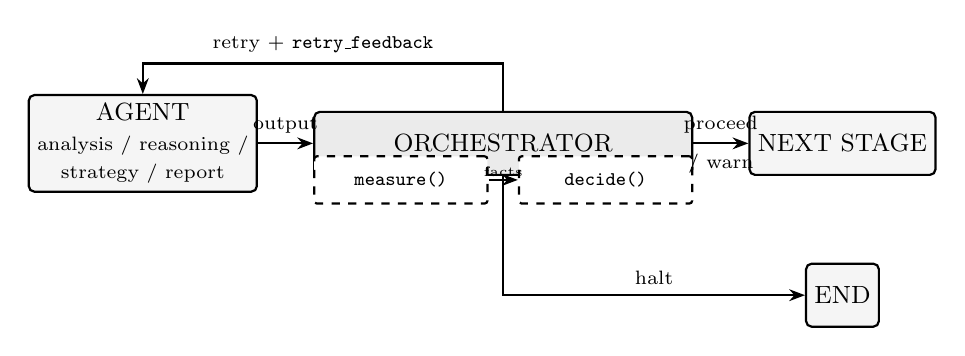
\begin{tikzpicture}[
  node distance=7mm,
  box/.style={draw, rounded corners=2pt, align=center, font=\small,
              minimum height=8mm, inner sep=3pt},
  agent/.style={box, fill=black!4, minimum width=22mm},
  orch/.style={box, fill=black!8, minimum width=48mm},
  sub/.style={draw, dashed, rounded corners=1pt, font=\scriptsize,
              minimum height=6mm, minimum width=22mm, fill=white},
  ->, >={Stealth[length=2mm]}, thick]

  \node[agent] (agent) {AGENT\\\scriptsize analysis / reasoning /\\[-1pt]
                        \scriptsize strategy / report};
  \node[orch, right=7mm of agent] (orch) {ORCHESTRATOR};
  \node[sub, below=1.5mm of orch.center, anchor=north, xshift=-13mm]
       (measure) {\texttt{measure()}};
  \node[sub, below=1.5mm of orch.center, anchor=north, xshift=13mm]
       (decide)  {\texttt{decide()}};
  \draw[->] (measure) -- node[above, font=\tiny, inner sep=1pt] {facts} (decide);

  \node[agent, right=7mm of orch] (next) {NEXT STAGE};
  \node[box, below=11mm of next, fill=black!4] (end) {END};

  \draw[->] (agent) -- node[above, font=\scriptsize] {output} (orch);
  \draw[->] (orch) -- node[above, font=\scriptsize] {proceed}
                      node[below, font=\scriptsize] {/ warn} (next);
  \draw[->] (orch.south) |- node[pos=0.75, above, font=\scriptsize] {halt} (end);

  \draw[->] (orch.north) -- ++(0,6mm) -| node[pos=0.25, above, font=\scriptsize]
       {retry $+$ \texttt{retry\_feedback}} (agent.north);
\end{tikzpicture}
\caption{One supervision cycle. The orchestrator measures the stage that just
ran with deterministic checks, then decides
\texttt{proceed\,|\,proceed\_with\_warning\,|\,retry\,|\,halt} by hard rules over
those measurements. A retry carries the measured failure back into the agent's
prompt. The supervisor makes no LLM call.}
\label{fig:hub}
\end{figure}
% ---------------------------------------------------------------------

\begin{table}[t]
\caption{Deterministic checks by stage. Every check resolves against upstream
state only; none consults an external oracle, a label set, or a language model.
The star rating used by the analysis contradiction check is the one supplied with
the review by its original author.}
\label{tab:checks}
\centering
\begin{tabular}{lp{7.6cm}}
\toprule
Stage & Measured facts \\
\midrule
Analysis  & Loaded vs.\ successfully analysed record counts; failure ratio and
            details; rate of contradiction between the review's own star rating
            and the predicted sentiment \\
Reasoning & Per pattern: evidence identifiers unresolvable against the analysis
            output; evidence whose aspect labels omit the pattern's aspect;
            claimed vs.\ independently recomputed frequency \\
Strategy  & Each recommendation's traceability to an upstream pattern or root
            cause, by string similarity \\
Report    & Root causes and recommendations not present upstream (containment);
            business-name and sample-size agreement with the pipeline's trusted
            values \\
\bottomrule
\end{tabular}
\end{table}


% =====================================================================

\section{Method}
\label{sec:method}

\subsection{Testbed and Data}

The testbed is the Yelp Open Dataset~\cite{yelpdataset}, a standard setting for
aspect-based sentiment
analysis~\cite{semeval2014,simmering2023,wu2024absa,niimi2024} and review
analytics over public corpora~\cite{malik2024}, in which we claim no
contribution; it is indexed by business in a local SQLite database built on
2026-08-03, and every figure below is measured against that index. Reviews are
drawn per business, so a run's input is one restaurant's review set rather than a
corpus slice and the system is evaluated on the unit it actually consumes. The
sampling pool is the 52{,}268 businesses carrying the \emph{Restaurants} category
and holding at least five reviews, five being the minimum below which the pipeline
declines to run. The per-business load cap was 214 reviews for every run, equal to
the largest stratum, so no sampled business was truncated and review count varies
only as the sampling design intends.

\subsection{Workload Sampling}
\label{sec:sampling}

Review count per restaurant is heavily skewed, so the sample is stratified across
it rather than drawn uniformly. Over the pool above the distribution runs
p10\,=\,7, p25\,=\,14, p50\,=\,34, p75\,=\,92, p90\,=\,214. A uniform draw would
concentrate on the high-$n$ tail and so describe a regime occupied by a tenth of
the population; stratifying at p25, p50, p75 and p90 spans the range the system
will meet, and makes incidence reportable \emph{as a function of} input size
rather than averaged over an unrepresentative mix.

Five businesses were drawn per stratum --- twenty in total, at 14, 34, 92 and 214
reviews respectively --- under a fixed seed. The sampler takes the businesses
whose review counts lie nearest each target percentile, so the strata are
controlled levels of the independent variable rather than sampled bands and
within-stratum variance is zero by construction. One feature of the measured
distribution bears on how the results should be read: with a low-confidence
threshold of 30 reviews, the median restaurant at 34 sits just above the system's
own confidence floor, so low-confidence warnings characterise the lower half of
the distribution rather than the typical case.


\subsection{Two-Phase Design}

The study runs in two phases over the same twenty businesses. In \textbf{Phase~A
(observe)} the supervisor measures every stage and records a verdict but always
proceeds; one run per business yields defect incidence under no intervention. In
\textbf{Phase~B (enforce)} only those businesses whose Phase~A run recorded a
retry-triggering defect are re-run with the verdict acted upon, yielding the rate
at which retry repairs what was detected.

Observe mode is the correct supervision-off arm because it differs from enforce
mode in exactly one respect --- whether the verdict is acted on. An earlier commit
or a different graph shape would confound supervision with architecture; the same
binary, same graph and same checks with enforcement disabled does not. Re-running
only the flagged businesses is justified because where nothing is detected the
arms are identical by construction: no retry fires, and the one remaining
difference --- the frequency overwrite of Section~\ref{sec:recompute} --- is
deterministic and computable from the Phase~A run alone.

\subsection{Repetition Sub-Study}
\label{sec:repetition}

The two-phase design assumes a defect observed once is present when the same
input is re-run. Phase~B put that in doubt, and five enforced runs cannot settle
it. Each of the five Phase~B businesses was therefore re-run five further times
in observe mode over identical input. The load cap exceeds every sampled
business, so each run reads that business's complete review set; with
temperature~0 this leaves provider non-determinism as the only varying quantity,
giving 25 independent observations of the same pipeline on the same data. Observe
mode is required here: the supervisor must measure without acting, or repetitions
would not be independent. Nothing else differs from Phase~A.

This estimates the per-run defect probability \emph{conditional on a defect
having been seen once}, which is the quantity the two-phase design assumes to be
near~1. Because the five businesses were selected on having shown a defect, the
resulting rates describe defect-prone workloads and are not population
estimates.

\subsection{Controls}

One provider and one model are fixed across both arms and recorded in each run's
configuration, at temperature~0 under a fixed sample seed. Two pre-existing
pipeline output dumps were deliberately \emph{not} reused as a before/after pair:
they ran on different providers, which would confound supervision with model
change. Temperature~0 constrains but does not eliminate non-determinism in a
hosted API, so no single-run difference is treated as significant; the claims
below rest on rates over the sample, not on individual pairs.

Runs remained subject to HTTP~503 provider failures and HTTP~429
credit-exhaustion errors, which the supervisor records as \texttt{status\_error}
facts. Such a fact reaches the same non-proceed verdict as a substantive grounding
defect, so it must be separated from one. The rule adopted here, fixed before any
figure in Section~\ref{sec:results} was computed, is that observations carrying a
\texttt{status\_error} fact are excluded from every incidence, rate and repair
count and reported instead as infrastructure loss. No affected run is repeated:
re-running only the subset that failed would make provider availability a
selection criterion.

The cost is small and concentrated. Three stage observations are lost across the
45 observe runs --- two in Phase~A, at the reasoning and report stages, and one in
the repetition sub-study, at the reasoning stage --- all on a single p90 business,
each an HTTP~503; Phase~B lost none. The exclusion removes no run from the sample,
so Table~\ref{tab:incidence} rests on 20 complete runs and the repetition figures
on 25. Because all three losses are non-proceed observations, excluding them can
only lower a reported defect rate, never raise one.

\subsection{Measures and Their Circularity}
\label{sec:measures}

The supervisor shares its check logic with the offline evaluator by design, so
that mid-run enforcement and after-the-fact scoring can never disagree about what
counts as ungrounded. That is sound engineering and a methodological trap, and it
belongs here rather than in Limitations because it bounds what the results may
claim: any improvement in a consistency-check score is close to tautological,
since enforcement optimises precisely the quantity that score reports.

Exactly one measure is circular in this sense --- the consistency-check delta ---
and it is reported for completeness alone. Four are not: Phase~A defect incidence
is descriptive, with no intervention applied; the Phase~B repair rate is not
guaranteed by construction and is the open question; token and latency overhead is
independent of what is enforced; and the independent judge
(Section~\ref{sec:judge}) uses a separate model and a rubric sharing no criterion
with the supervisor's checks. The headline claim rests on those four.

% =====================================================================
\section{Results}
\label{sec:results}

Twenty businesses completed Phase~A and the five that recorded a retry-triggering
defect completed Phase~B. Two stage observations were excluded as infrastructure
loss (Section~\ref{sec:method}), leaving 78 of 80 in Phase~A.

\subsection{Defect Incidence}

At least one grounding defect appeared in \textbf{7 of 20 runs (35\%)}, across 13
instances; including the by-definition low-sample flag raises this to 11 of 20
(55\%). The decomposition in Table~\ref{tab:incidence} matters more than the
aggregate. Three of the eight checks never fired, but two of those zeros are
artefacts of measuring once per business --- unresolvable evidence identifiers and
unsupported report content both appear under repetition
(Section~\ref{sec:repetition}) --- so the table records what these twenty draws
contained, not what the pipeline can produce. Defects concentrated instead in
untraceable recommendations and star/sentiment contradictions, each in 3 of 20
runs.

The statistic-divergence row shows why businesses affected and total instances
must be reported separately. Six divergent frequency claims occurred, but all six
came from a single business; nineteen produced none. Read as ``5\% of runs'' the
finding looks marginal, and read as six instances it looks systemic; it is
neither. It is one workload in which the reasoning stage misestimated every
frequency it asserted --- a workload-level anomaly, not a model-level tendency.

\begin{table}[t]
\caption{Defects detected in observe mode (Phase A), by check type. $n=20$ runs;
two stage observations excluded as infrastructure loss.}
\label{tab:incidence}
\centering
\begin{tabular}{lrrr}
\toprule
Check & Businesses affected & Instances & \% of runs \\
\midrule
Unresolvable evidence ID      & 0 & 0 & 0 \\
Misaligned aspect             & 1 & 1 & 5 \\
Statistic divergence          & 1 & 6 & 5 \\
Star/sentiment contradiction  & 3 & 3 & 15 \\
Untraceable recommendation    & 3 & 3 & 15 \\
Unsupported report content    & 0 & 0 & 0 \\
Metadata mismatch             & 0 & 0 & 0 \\
Low sample size               & 5 & 5 & 25 \\
\midrule
\textbf{Any grounding defect} & \textbf{7} & \textbf{13} & \textbf{35} \\
Any defect, incl.\ low sample & 11 & 18 & 55 \\
\bottomrule
\end{tabular}
\end{table}

\subsection{Does Defect Rate Track Sample Size?}

Separating the low-sample flag --- which fires by definition below 30 reviews and
therefore on the p25 stratum alone --- leaves the grounding defects free to vary.
They do not vary smoothly. Mean grounding instances per run are 0.2 at each of
p25, p50 and p75, then rise tenfold to 2.0 at p90 (Fig.~\ref{fig:rate-vs-n}). The
flat region spans a sixfold increase in input size, so this is not a dose
response; it is a threshold effect somewhere above 92 reviews, and the largest
single contributor is the one business discussed above. The direction is
informative even though the sample cannot locate the threshold: grounding defects
here are workload-driven rather than uniformly model-driven, and a supervisor
calibrated on median-sized inputs would be calibrated on the regime where almost
nothing happens.

This trend rests on one run per business, which is a noisy estimate: across five
identical repeats, individual businesses ranged 0--3, 0--6 and 1--7 defects
(Section~\ref{sec:repetition}). The direction is nonetheless consistent under
repetition --- the three repeated p90 businesses averaged 1.8, 2.0 and 5.4 defects
per run against 0.0 for the repeated p50 business --- but those five were selected
for having shown a defect and so cannot confirm a stratum mean; the magnitude of
the p90 rise is indicative rather than measured.

\begin{figure}[t]
\centering
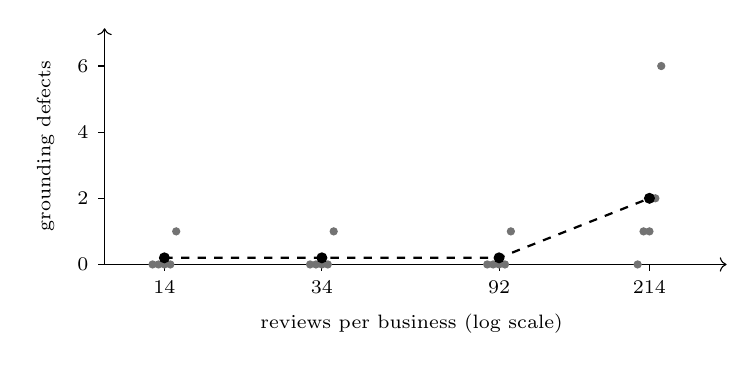
\begin{tikzpicture}[x=1cm,y=1cm]
  \draw[->] (0,0) -- (7.9,0);
  \draw[->] (0,0) -- (0,3.0);
  \foreach \x/\l in {0.76/14, 2.76/34, 5.01/92, 6.92/214}
    \draw (\x,0) -- (\x,-0.08) node[below,font=\scriptsize] {\l};
  \foreach \y/\l in {0/0, 0.84/2, 1.68/4, 2.52/6}
    \draw (0,\y) -- (-0.08,\y) node[left,font=\scriptsize] {\l};
  \node[below,font=\scriptsize] at (3.9,-0.5) {reviews per business (log scale)};
  \node[rotate=90,font=\scriptsize] at (-0.75,1.5) {grounding defects};
  % individual runs
  \foreach \p in {(0.61,0),(0.685,0),(0.76,0),(0.835,0),(0.91,0.42),
                  (2.61,0),(2.685,0),(2.76,0),(2.835,0),(2.91,0.42),
                  (4.86,0),(4.935,0),(5.01,0),(5.085,0),(5.16,0.42),
                  (6.77,0),(6.845,0.42),(6.92,0.42),(6.995,0.84),(7.07,2.52)}
    \fill[black!55] \p circle (1.5pt);
  % stratum means
  \draw[dashed,thick] (0.76,0.084) -- (2.76,0.084) -- (5.01,0.084) -- (6.92,0.84);
  \foreach \p in {(0.76,0.084),(2.76,0.084),(5.01,0.084),(6.92,0.84)}
    \fill \p circle (2pt);
\end{tikzpicture}
\caption{Grounding defects per run against review count, with the by-definition
low-sample flag excluded. Dots are individual runs (jittered horizontally); the
dashed line joins stratum means. The rate is flat across a sixfold increase in
input size and rises only at p90.}
\label{fig:rate-vs-n}
\end{figure}

\subsection{Does Feedback-Injected Retry Repair the Defect?}

Phase~B fired a single retry across five businesses --- ambiguous on its own,
since either detected defects almost never recur or the arm was too small to
contain them. The repetition sub-study separates the two.

Defects recur; \emph{retry-triggering} defects recur rarely. Across 25 repetitions
some defect was present in 17 runs (68\%), but only 8 (32\%) reached a
\texttt{retry} verdict, because the two most frequent classes never produce one:
star/sentiment contradiction ran near 0.5\%, far beneath the 20\% ceiling, and
statistic divergence is resolved by overwrite rather than regeneration. The defect
Phase~A recorded reappeared at the same stage in only 5 of 25 runs (20\%), and the
affected stage itself moved: one business flagged at strategy in Phase~A retried
at reasoning in two repetitions and at strategy in none (Table~\ref{tab:repair}).

At a per-run retry rate of 0.32, a five-business enforce arm should yield about
1.6 retries. It yielded 1. \textbf{Phase~B was therefore underpowered rather than
anomalous}, and the repair rate remains unmeasured. Measuring it requires roughly
an order of magnitude more enforced runs, or a harness that injects
known-defective stage outputs directly rather than waiting for a stochastic defect
to appear.

The instability is itself the substantive finding. On identical input, at
temperature~0, this pipeline does not merely vary in whether it emits a defect; it
varies in \emph{which stage} emits one. Any evaluation that runs a staged LLM
system once per input and reports the defects it happened to catch is reporting a
draw, not a property --- and a supervisor tuned against a single run is tuned
against noise.

\begin{table}[t]
\caption{Recurrence of retry-triggering defects across five observe-mode
repetitions per business, on input identical to Phase~A.}
\label{tab:repair}
\centering
\begin{tabular}{llrrr}
\toprule
Business & Phase~A stage & Runs & Any retry & Same stage \\
\midrule
Red Lobster       & strategy          & 5 & 0 & 0 \\
Izzo's            & strategy          & 5 & 3 & 3 \\
Nomzilla!         & reasoning         & 5 & 2 & 2 \\
Ameristar         & strategy          & 5 & 2 & 0 \\
Scarpetta         & (provider error)  & 5 & 1 & 0 \\
\midrule
\textbf{Total}    &                   & \textbf{25} & \textbf{8 (32\%)} & \textbf{5 (20\%)} \\
\bottomrule
\end{tabular}
\end{table}

\subsection{Cost of Supervision}

The supervisor makes no model call, so any token overhead is attributable to
retries and all remaining overhead is local computation. The latency consequence
is \emph{below what this study can resolve}: mean wall-clock was 597.3\,s over the
25 observe repetitions against 566.5\,s over the five enforced runs, so
enforcement measured 5.2\% \emph{faster}. That is the noise floor becoming
visible, not a speed-up --- wall-clock varies by 9.4\% within a business across
identical repeated runs, and one business ranged from 696\,s to 1105\,s. Five runs
against five cannot resolve an effect smaller than that, and an earlier reading
comparing one observe run against one enforced run produced a spurious $+0.2$\%
overhead. The bounded claim that survives: with one retry fired across five
enforced runs, supervision introduced no latency cost detectable above run-to-run
variance, consistent with checks that are deterministic Python over state already
in memory.

\subsection{Independent Judge Assessment}
\label{sec:judge}

Section~\ref{sec:measures} obliges at least one quality measure the supervisor
does not define. A separate model
(\texttt{gemini-3.1-pro-\allowbreak preview}, a different generation and tier from the
\texttt{gemini-2.5-flash} under test) scored both arms' reports against a rubric
sharing nothing with the supervisor's checks: actionability, specificity,
coherence and restraint. Everything the supervisor enforces is absent from it by
construction.

Each pair was judged blind, with arm-to-position assignment alternated so a
positional preference could not be read as a quality difference, and repeated
three times. Four of the five Phase~B businesses contribute: the fifth is excluded
because provider failure left its observe-arm report empty. That yields 12
verdicts over 4 pairs.

\textbf{Enforcement produced no measurable quality difference}
(Table~\ref{tab:judge}). The overall means are 2.65 observe against 2.60 enforce,
a delta of $-0.04$ on a five-point scale against a within-arm standard deviation
of roughly 0.8; three of the four dimensions are identical to two decimal places.
Preference splits 5 enforce, 4 observe, 3 tie. This is the expected result: only
one of the four pairs had a retry fire at all, so three of them are two draws from
the same unsupervised process, and the null is mostly a measurement of judge
noise. We claim no significance from four pairs.

Two observations survive the null. The absolute scores are informative
independently of the comparison: both arms score 3.7--3.8 on coherence but only
2.2--2.3 on actionability, specificity and restraint, so an independent reader
finds these reports internally consistent yet generic and prone to asserting more
than the reviews support --- a deficiency groundedness checking cannot reach.
Second, the judge showed a position effect large enough to have manufactured a
result under a fixed order (Section~\ref{sec:discussion}).

\begin{table}[t]
\caption{Independent judge scores (1--5, higher is better), 12 verdicts over 4
blind counterbalanced pairs, three repetitions each.}
\label{tab:judge}
\centering
\begin{tabular}{lrrr}
\toprule
Dimension & Observe & Enforce & Delta \\
\midrule
Actionability & 2.33 & 2.33 & $+0.00$ \\
Specificity   & 2.25 & 2.25 & $+0.00$ \\
Coherence     & 3.83 & 3.67 & $-0.17$ \\
Restraint     & 2.17 & 2.17 & $+0.00$ \\
\midrule
\textbf{Overall} & \textbf{2.65} & \textbf{2.60} & $\mathbf{-0.04}$ \\
\multicolumn{4}{l}{Preference: 5 enforce, 4 observe, 3 tie. Within-arm sd $\approx 0.8$.} \\
\bottomrule
\end{tabular}
\end{table}

\subsection{A Caught Defect}
\label{sec:caught}

One business asserted six pattern frequencies and overstated every one of them:
0.63 against a recomputed 0.39 for food quality, 0.49 against 0.27 for staff
attitude, and four more in the same direction, each inflated by a factor between
1.6 and 1.8. The claims were internally consistent, correctly ranked, and
individually plausible; nothing in the schema was violated and no evidence
identifier was wrong. Only recomputation exposed them, and because the frequency
is a quantity the checker can derive, the supervisor overwrote all six rather
than retrying (Section~\ref{sec:recompute}) --- the defect was deleted rather than
detected, at zero model cost. This is the mildest possible failure: prose that
would have read as authoritative to any human reviewer, wrong only in its
arithmetic, in a system whose schema validation passed.

% =====================================================================
\section{Discussion, Limitations, and Threats to Validity}
\label{sec:discussion}

\subsubsection{Circularity.}
The supervisor shares its check definitions with the offline harness it was
derived from, so any improvement in the consistency-check score under enforcement
is close to tautological. We exclude that score from every claim in this paper;
the results rest on the four non-circular measures of
Section~\ref{sec:measures}.

\subsubsection{Detection is not adjudication.}
The mechanism sees missing provenance, not falsehood: an unsupported claim may be
true, an accepted claim may inherit an upstream error, and defects originating in
the analysis stage are invisible except where the data carries an independent
signal, as the star ratings do. Every incidence figure in
Section~\ref{sec:results} is therefore a lower bound on ungrounded content, not
an estimate of total error.

\subsubsection{Derivability is a precondition, not a universal.}
The pattern transfers to pipelines whose stages read only what earlier stages in
the same run produced. It does not transfer to architectures admitting inputs the
supervisor cannot see: shared scratchpads or blackboards, retrieval or tool calls
in the loop, memory carried across runs, or free-form conversational agents where
provenance is not structural. The requirement is closure rather than linearity,
but closure is a real constraint that many deployed agent systems violate.

\subsubsection{Single domain, dataset, and provider.}
All runs use one pipeline, one public dataset, and one provider and model held
fixed and recorded per run. The two-arm design controls for the provider; it does
not test across providers. The rates reported are properties of a system, not of
language models.

\subsubsection{Thresholds are uncalibrated proposals.}
The minimum viable sample, low-confidence cutoff, contradiction ceiling,
frequency tolerance, trace similarity threshold, and retry cap are engineering
choices --- none derived from the literature, none tuned against held-out data.
Their effect is direct: a different contradiction ceiling yields a different
incidence figure. We therefore report which check produced each detection rather
than only the aggregate. This study's data is the first calibration input these
thresholds have had.

\subsubsection{Reference labels are thin.}
Human-labelled data exists for a single business, annotated by one person, so
inter-annotator agreement is uncomputed and the labels cannot support an accuracy
claim; we use them for calibration only. This limits what the paper can say about
whether the analysis stage is \emph{correct}, as distinct from whether downstream
stages stay within it.

\subsubsection{Judge bias and sample size.}
The independent-judge measure inherits the known failure modes of LLM
evaluators~\cite{positionbias,selfpreference}; we treat it as indicative rather
than decisive. The sample is stratified to span a distribution, not powered to
detect a difference, so proportions are reported with denominators visible and are
not population estimates.

The counterbalancing of Section~\ref{sec:judge} proved necessary: of the nine
verdicts that were not ties, seven favoured whichever report happened to be shown
first --- a position effect larger than the difference between the arms it was
meant to measure. A fixed-order judge would have manufactured a result here, and
we recommend against running one.

Proportions are reported with Wilson 95\% intervals, which at these denominators
are wide enough to be worth stating explicitly: grounding-defect incidence
35\% (7/20, CI 18--57\%), any defect including the low-sample flag 55\% (11/20,
CI 34--74\%), a retry-triggering defect under repetition 32\% (8/25, CI
17--52\%), and recurrence at the same stage 20\% (5/25, CI 9--39\%). No claim
here rests on separating any two of these figures. They are reported to
establish that the defect class occurs at a rate worth engineering against,
which the lower bounds alone support.

% =====================================================================
\section{Conclusion}
\label{sec:conclusion}

The transferable result is a property, not a system. When every agent in a
pipeline reads only what earlier agents in the same run produced, groundedness
becomes decidable against the pipeline's own state, so an evaluation harness ---
ordinarily an offline artefact --- can hold the control path at run time, at zero
model calls and with a reproducible, auditable verdict. The restaurant review
pipeline is where we measured this; it is not what the result is about.

Two numbers carry the empirical weight, and only one is strong. A grounding defect
appeared in seven of twenty unsupervised runs, which places ungrounded output in
ordinary operation rather than at the edges. The enforcing arm produced a single
retry, far too few to estimate a repair rate, so we claim only that the defects
are detected and that the arm was underpowered rather than anomalous. The
repetition study did establish that a defect recurs at the same stage in one run
in five, so a single evaluation run of a staged pipeline reports a draw rather
than a property --- whether or not supervision is switched on. The immediate
extension is to attach an interval to each recomputed frequency and propagate it
into the report: exactness is not confidence, and the supervisor already holds
every quantity this requires.

% =====================================================================
\bibliographystyle{splncs04}
\bibliography{references}

\end{document}